
\documentclass[calculator,allquestions,datasheet,mock,solutions]{exam_newMarcus2}
%\documentclass[calculator,allquestions,datasheet,mock,Pens]{exam_newMarcus2}

% The full list of class options are
% calculator : Allows approved calculator use.
% datasheet : Adds a note that data sheet are attached to the exam.
% handbook : Allows the use of the engineering handbook.
% resit : Adds the resit markings to the paper.
% sample : Adds conspicuous SAMPLE markings to the paper
% solutions : Uses the contents of \solution commands (and \solmarks) to generate a solution file
% mock: For a mock-exam paper

\usepackage{pdfpages}  
\usepackage{lscape,comment} 
 
\coursecode{EX3029}%%
\coursetitle{Chemical Thermodynamics}
 
\examtime{14.00--16.00}%
\examdate{16}{11}{2017}% 
\examformat{Attempt ALL questions. \\ Each question is worth 20 marks.}

% Other symbols
\newcommand{\frc}{\displaystyle\frac}
\newcommand{\br}[1]{\!\left( #1 \right)}
\newcommand{\abs}[1]{\left| #1 \right|}
\newcommand{\fracd}[2]{\frac{\mathrm{d} #1}{\mathrm{d} #2}}
\newcommand{\fracp}[2]{\frac{\partial #1}{\partial #2}}
\renewcommand{\d}[1]{\mathrm{d} #1 } 
\newcommand{\Ma}{\mathrm{M\!a}} 
\newcommand{\eg}{{\it e.g., }}
\newcommand{\ie}{{\it i.e., }}
\newcommand{\wrt}{{\it wrt }}
\newcommand{\Partial}[3][error]{\left(\frc{\partial #1}{\partial #2}\right)_{#3}}
\newcommand{\mfr}[3][error]{#1_{#2}^{\left(#3\right)}} 
\newcommand{\summation}[3][error]{\sum\limits_{#2}^{#3}#1} 

\begin{document}


%%%
%%% Question 01
%%%
\begin{question}
\begin{enumerate}[(a)]
%
\item Derive the Maxwell relations below from the fundamental thermodynamic equations.~\marks{11}
\begin{eqnarray}
 \left(\frac{\partial T}{\partial V}\right)_{S} = -\left(\frc{\partial P}{\partial S}\right)_{V}; && 
 \left(\frc{\partial T}{\partial P}\right)_{S} = \left(\frac{\partial V}{\partial S}\right)_{P}; \nonumber \\
 \left(\frc{\partial P}{\partial T}\right)_{V} = \left(\frac{\partial S}{\partial V}\right)_{T}; &&%
  \left(\frac{\partial V}{\partial T}\right)_{P} = -\left(\frc{\partial S}{\partial P}\right)_{T} \nonumber 
\end{eqnarray}
%==========================
%
\solution{First, let's assume a functional $f=f\left(a,b\right)$ and rewrite it as a function of the variables $a$ and $b$,~\solmarks{1/11}
\begin{displaymath}
df = \left(\frc{\partial f}{\partial a}\right)_{b}da + \left(\frc{\partial f}{\partial b}\right)_{a}db
\end{displaymath}
If we define $M=\left(\frc{\partial f}{\partial a}\right)_{b}$ and $N=\left(\frc{\partial f}{\partial b}\right)_{a}$, the equation above becomes~\solmarks{1/11}
\begin{equation}
{\bf df = M da + N db}\label{eqn1}
\end{equation}
Now, if we differentiate $M$ and $N$ with respect to $b$ and $a$, respectively,~\solmarks{1/11}
\begin{displaymath}
\left(\frc{\partial M}{\partial b}\right)_{a} = \frc{\partial^{2} f}{\partial a\partial b}\;\;\text{ and }\;\;\left(\frc{\partial N}{\partial a}\right)_{b} = \frc{\partial^{2} f}{\partial b\partial a}
\end{displaymath}
If the functional $f$ is continuous and differentiable over all domain,~\solmarks{1/11}
\begin{equation}\label{eqn2}
\frc{\partial^{2} f}{\partial a\partial b} = \frc{\partial^{2} f}{\partial b\partial a} \Longrightarrow {\bf \left(\frc{\partial M}{\partial b}\right)_{a} = \left(\frc{\partial N}{\partial a}\right)_{b} }
\end{equation}
The fundamental thermodynamic relations,~\solmarks{1/11} 
\begin{eqnarray}
&& dU = - PdV + TdS \nonumber \\ 
&& dH =   TdS + VdP \nonumber \\
&& dA = - PdV - SdT \nonumber \\
&& dG = - VdP - SdT \nonumber
\end{eqnarray}
have similar shape as Eqn.~\ref{eqn1}, where, for example, in the first relation: ~\solmarks{1/11} 
   \begin{displaymath}
     U = f,\; M=-P,\; N=T,\; \d V=\d a\;\text{ and }\; \d S=\d b. 
   \end{displaymath}
Using relation~\ref{eqn2},~\solmarks{2/11}
   \begin{displaymath}
         -\left(\frc{\partial P}{\partial S}\right)_{V}=\left(\frc{\partial T}{\partial V}\right)_{S}.
   \end{displaymath}
Applying the same to the remaining relations we obtain:~\solmarks{3/11}
\begin{displaymath}
 \left(\frc{\partial T}{\partial P}\right)_{S} = \left(\frac{\partial V}{\partial S}\right)_{P},\; \left(\frc{\partial P}{\partial T}\right)_{V} = \left(\frac{\partial S}{\partial V}\right)_{T}, \text{ and }\; \left(\frac{\partial V}{\partial T}\right)_{P} = -\left(\frc{\partial S}{\partial P}\right)_{T} 
\end{displaymath}
}
%
\item Using the Maxwell relations above, evaluate $\left(\frc{\partial S}{\partial V}\right)_{T}$ for water vapour at 240$^{\circ}$C and molar volume of 0.0258 m$^{3}$ mol$^{-1}$ through the Redlich-Kwong equation of state,
\begin{displaymath}
P = \frc{RT}{V-b} - \frc{a}{V\left(V+b\right)T^{1/2}}
\end{displaymath}
with 
$R$ = 8.314$\times$ 10$^{-5}\;\text{bar m}^{3} \left(\text{mol K}\right)^{-1}$, $a$ = 142.59 $\times$ 10$^{-6}\;\text{bar m}^{6} \left(\text{mol K}\right)^{-2}$ and $b$ = 0.0211 $\times$ 10$^{-3}\text{m}^{3}\;\text{mol}^{-1}$.~\marks{9}


%\frc{\text{bar.m}^{3}}{\text{mol.K}}$, $a$ = 142.59 $\times$ 10$^{-6}\; \frc{\text{bar.m}^{6}}{\left(\text{mol.K}\right)^{2}}$ and $b$ = 0.0211 $\times$ 10$^{-3}\frc{\text{m}^{3}}{\text{mol}}$.~\marks{9}
%==========================
\solution{The Maxwell relation ~\solmarks{2/9}
   \begin{displaymath}
      \left(\frc{\partial P}{\partial T}\right)_{V} = \left(\frc{\partial S}{\partial V}\right)_{T}
   \end{displaymath}
    allows to determine $\left(\frc{\partial S}{\partial V}\right)_{T}$ from the PVT relationship in the RK EOS. Thus,~\solmarks{4/9}
\begin{displaymath}
{\bf \left(\frc{\partial P}{\partial T}\right)_{V} = \frc{R}{V-b} + \frc{a}{2 V\left( V + b \right)T^{\frac{3}{2}}}}
\end{displaymath}
Now substituting the variables by their values~\solmarks{3/9}
\begin{displaymath}
  \left(\frc{\partial P}{\partial T}\right)_{V} = \left(\frc{\partial S}{\partial V}\right)_{T} = 3.2342\times 10^{-3} \text{bar.K}^{-1} = 3.2342\times 10^{-1}\frc{\text{kJ}}{\text{m}^{3}.\text{K}}
\end{displaymath}

}
%
\end{enumerate}

\end{question}

\clearpage




%%%
%%% Question 02
%%%
\begin{question}

   Scientists in China are investigating the feasibility of a novel enhanced geothermal system (EGS) technology to produce power and heat in the Gonghe basin in the northwestern province of Qinghai. Their initial well test demonstrated that at a depth of 3705 meters, the geological formation temperature is of 235$^{\circ}$C.  They predicted that 5.6805 kg.s$^{-1}$ of brine $\left(m_{\text{br}}\right)$ can be extracted from the reservoir and, at the top of the well, pressure and temperature of the fluid are 15 bar and 200$^{\circ}$C, respectively. In their preliminary plant design (Fig.~\ref{Figure:Fig1}), 2 turbines would produce 3.5 MW of power, whilst a condenser (fed with cold water, A) would extract 15.75 MW of heat from the brine before re-injection into the geothermal reservoir. 
      \begin{figure}[h]
        \begin{center}
          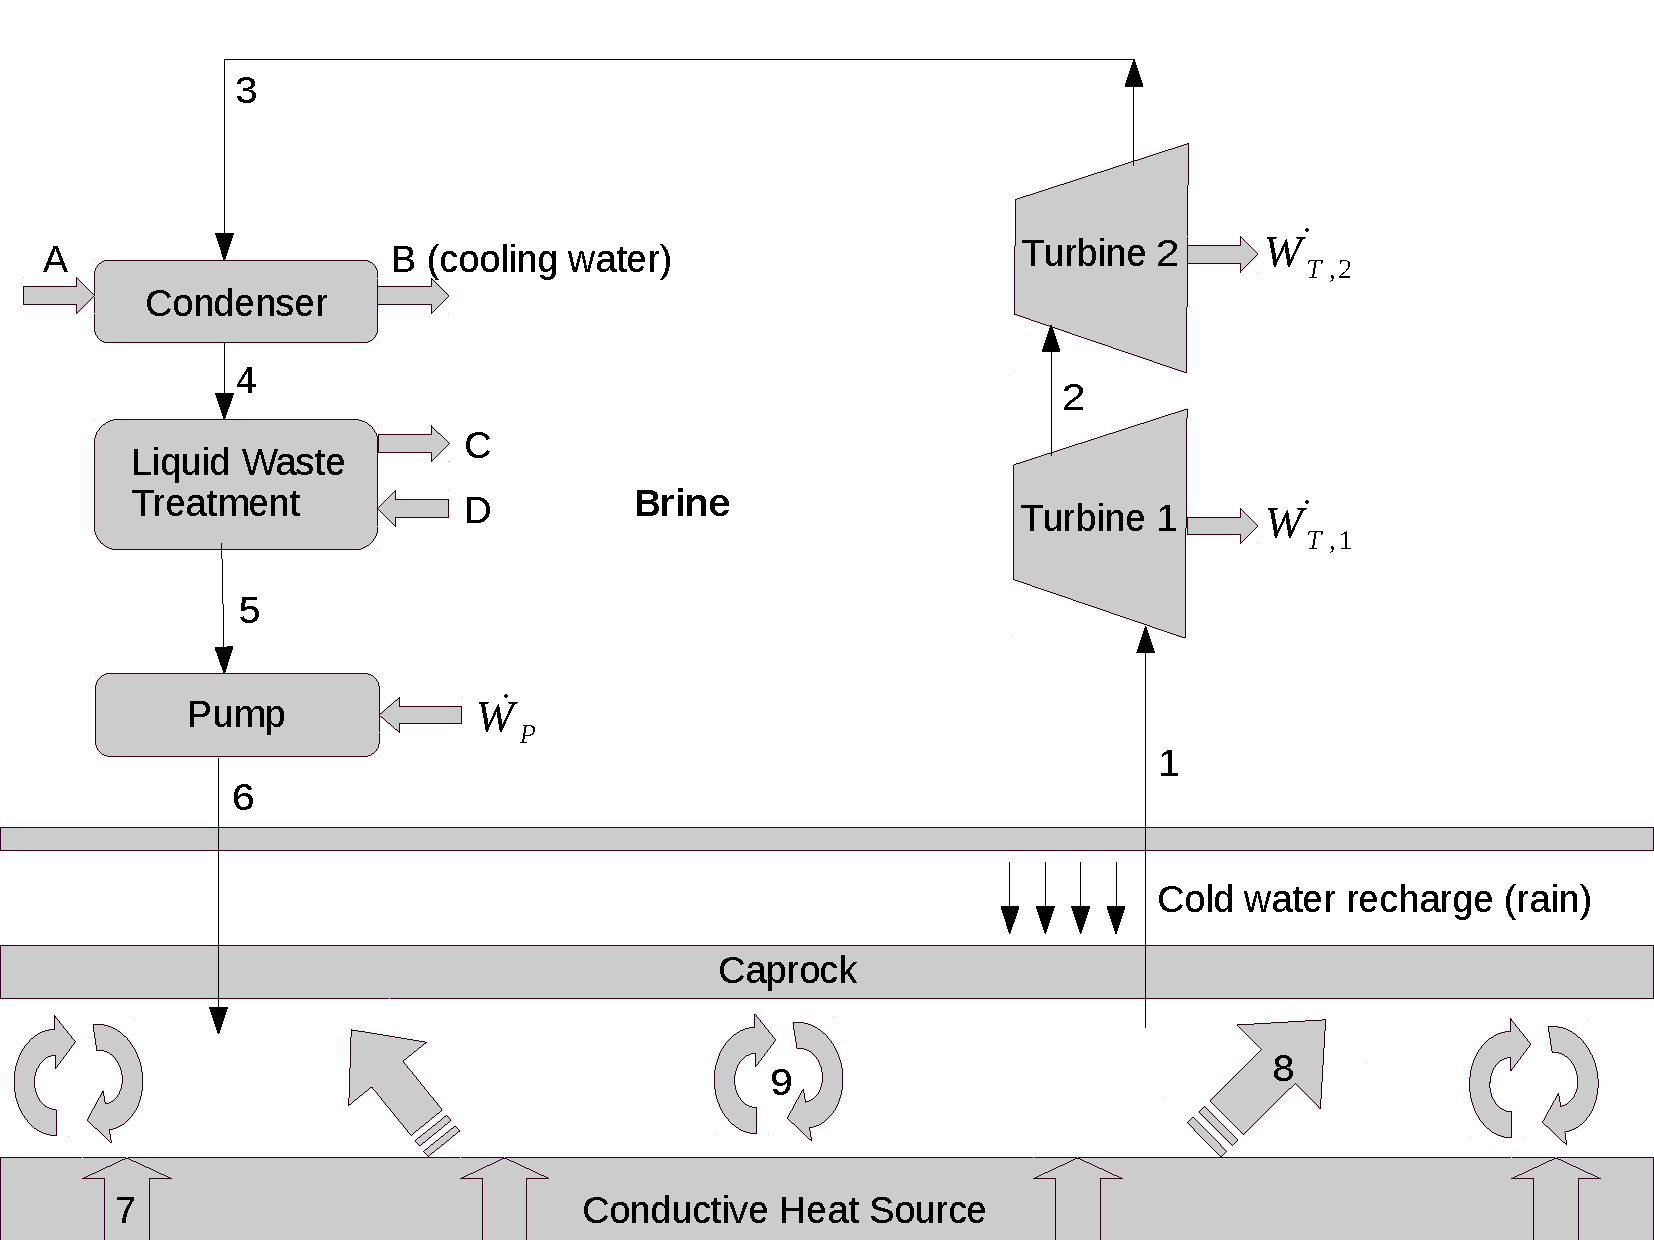
\includegraphics[width=.8\linewidth,clip]{./Pics/Exam2_PowerPorousMedia.pdf}
          \caption{Schematics of geothermal source exploration for power and heat production.}\label{Figure:Fig1}
        \end{center}
      \end{figure}
      
      \begin{table}[h]
        \begin{center}
          \begin{tabular}{||c|c|c|c|c|c||}
            \hline\hline
                {\bf Stream} & {\bf Pressure} & {\bf Temperature} & {\bf Fluid} & {\bf Specific enthalpy} & {\bf Specific entropy} \\
                             & {\bf (bar)}    & {\bf $\left(^{\circ}\text{C}\right)$}& &  {\bf $\left(\text{kJ.kg}^{-1}\right)$} & {\bf $\left(\text{kJ.kg}^{-1}\text{.K}^{-1}\right)$} \\  
            \hline\hline
                {\bf 1}      &   15           &   200              & (i)        &  (ii)                   &   (iii)                  \\
            \hline
                {\bf 2}      &   7            &   180              & dry vapour &   (iv)                  &   (v)                     \\ 
            \hline
                {\bf 3}      &   5            &   --               & (vi)       &   (vii)                 &    (viii)                 \\
            \hline
                {\bf 4}      &   --           &   (ix)             & --        &    (x)                   &    --                     \\
            \hline
                {\bf 5}      &   4.50         &   147.90           & --        &    (xi)                  &    --                     \\
            \hline
                {\bf 6}      &   25.00        &   --               & (xii)      &    (xiii)               &    --                     \\
            \hline
                {\bf A}      &   --           &   20               & Cold water  &   --                   &    --                     \\
            \hline
                {\bf B}      &   --           &   --               & Hot water  &   --                   &    --                     \\
            \hline
                {\bf C}      &   --           &   --               & Liquid residue&   --                   &    --                     \\
            \hline
                {\bf D}      &   --           &   --               & Cold water  &   --                   &    --                     \\
            \hline\hline
          \end{tabular}
           \caption{Thermal-physical​ conditions​ ​of​ all​ streams​ ​from​ ​Fig.​~\ref{Figure:Fig1}}\label{Table:Tab1}
        \end{center}
      \end{table}

       Before re-injection, contaminants are removed from the brine stream at a rate of 0.1 kg.s​$^{-1}$ (stream C) and, in order to replenish the geothermal reservoir, 10 kg.s​$^{-1}$ of cold water is added into the brine stream (D). Your task is to check if the predicted power and heat production are correct, therefore: 
  \begin{enumerate}[a)]
     \item Calculate conditions (i-xiii) from Table~\ref{Table:Tab1};~\marks{13}
         \solution{Following the streams:
            \begin{enumerate}[1)]
               \item At $P_{1}=15$ bar and $T_{1}=200^{\circ}$C, brine is at {\it superheated vapour} state {\bf (i)}\solmarks{1/13} with $h_{1}=2796.8\text{ kJ.kg}^{-1}$ {\bf (ii)}\solmarks{1/13} and $s_{1}=6.4546\text{ kJ.kg}^{-1}$ {\bf (iii)}\solmarks{1/13};
               \item At $P_{2}=7$ bar, brine is a dry vapour with $h_{2}=2763.5\text{ kJ.kg}^{-1}$ {\bf (iv)}\solmarks{1/13} and $s_{2}=6.7080\text{ kJ.kg}^{-1}$ {\bf (v)}\solmarks{1/13};
               \item At $P_{3}=5$ bar, an isentropic expansion of the fluid occurs in Turbine 2, \ie $s_{3}=s_{2}=6.7080\text{ kJ.kg}^{-1}$ {\bf (viii)}\solmarks{1/13}. At such pressure, the saturation table gives:
                 \begin{displaymath}
                   \begin{cases}
                      h_{f} = 640.23\text{ kJ.kg}^{-1}, & s_{f} = 1.8607\text{ kJ.(kg.K)}^{-1}, \\
                      h_{g} = 2748.7\text{ kJ.kg}^{-1}, & s_{g} = 6.8212\text{ kJ.(kg.K)}^{-1}.
                   \end{cases}
                 \end{displaymath}
                 As $s_{3}<s_{g}$, the fluid is {\it wet vapour} {\bf (vi)}~\solmarks{1/13}. In order to calculate the enthalpy of this stream, we first need​​ to obtain the quality​ of the vapour through,\solmarks{1/13}
                 \begin{displaymath}
                   \begin{cases}
                     x_{3} = \frc{s_{3}-s_{f}}{s_{g}-s_{f}} = 0.9772, & \\
                     x_{3} = \frc{h_{3}-h_{f}}{h_{g}-h_{f}} & \Longrightarrow h_{3} = 2700.626 \text{ kJ.kg}^{-1}\textbf{ (vii)}
                   \end{cases}
                 \end{displaymath}
               \item The condenser removes heat from the brine stream with no pressure drop, therefore $P_{4}=P_{3}=5$ bar with $T_{4}=T_{\text{sat}}=151.9^{\circ}$C {\bf (ix)}~\solmarks{1/13}. Fluid leaving the condenser is saturated liquid with $h_{4}=h_{f}=640.23\text{ kJ.kg}^{-1}$ {\bf (x)}\solmarks{1/13};
               \item After the liquid waste treatment unit, the brine stream is at $P_{5}=4.5$ bar and the saturated temperature is $T_{\text{sat}}=T_{5}=147.9^{\circ}$C, thus the brine is at saturated liquid state with $h_{5}=623.25\text{ kJ.kg}^{-1}$ {\bf (xi)}\solmarks{1/13} and $v_{5}=1.0882\times 10^{-3}\text{ m}^{3}\text{.kg}^{-1}$;
               \item At the pump, $P_{6}=25$ bar, the fluid undertakes an isentropic compression and from the fundamental thermodynamic relation:
                   \begin{displaymath}
                      Tds = dh - vdP.
                   \end{displaymath}
                   However, as $ds = 0$ (\ie isentropic) and, assuming that the fluid is incompressible, \ie $v_{6}=v_{5}$,~\solmarks{1/13}
                   \begin{displaymath}
                      \int dh = \int vdP \;\;\Longrightarrow h_{6}=h_{5} + v_{5}\left(P_{6}-P_{5}\right) = 625.4808\text{ kJ.kg}^{-1} \text{\bf  (xiii)}.
                   \end{displaymath}
                    At 25 bar, the saturated liquid enthalpy, $h_{f}$, is 962.11 kJ.kg$^{-1} > h_{6}$, therefore the brine is at {\it subcooled liquid state} {\bf (xii)}. ~\solmarks{1/13}
            \end{enumerate}
         }
%%%%%%%%%%%%%%%%%%%%%%       
       \item Are the predictions of power and heat correct? If not, calculate the power produced by the Turbines and heat extracted by the Condenser;~\marks{3}
         \solution{ Total power produced by the turbines are~\solmarks{1/3}
           \begin{eqnarray}
              \dot{W}_{T} &=& \dot{W}_{T,1} + \dot{W}_{T,2} =  \dot{m}_{br}\left(h_{2}-h_{1}\right) + \dot{m}_{br}\left(h_{2}-h_{1}\right) \nonumber \\
                         &=& -546.30\text{kJ.kg}^{-1} =  0.5463\text{ MW} \nonumber
           \end{eqnarray}
           The heat extracted by the condenser is~\solmarks{1/3}
              \begin{displaymath}
                  \dot{Q}_{c} = \dot{m}_{br}\left(h_{4}-h_{3}\right) = -11704.4771\text{ kJ.kg}^{-1} = 11.7045\text{ MW}
              \end{displaymath}
              Thus, scientists over-predicted power production and heat extraction from the power plant~\solmarks{1/3}.
           }
     \item Sketch the temperature $\times$ specific entropy $\left(Ts\right)$ diagram of the process involving streams (1)-(4), indicating:~\marks{4}
       \begin{itemize}
          \item entropies and temperatures;
          \item liquid saturated line;
          \item vapour saturated line;
          \item critical point;
          \item isobars.
       \end{itemize}
       \solution{
         Marks:
         \begin{itemize}
            \item entropies and temperatures;\solmarks{2/4}
          \item liquid and vapour saturated line;\solmarks{1/4}
          \item isobras and critical point.\solmarks{1/4}
         \end{itemize}
         
        \begin{center}
          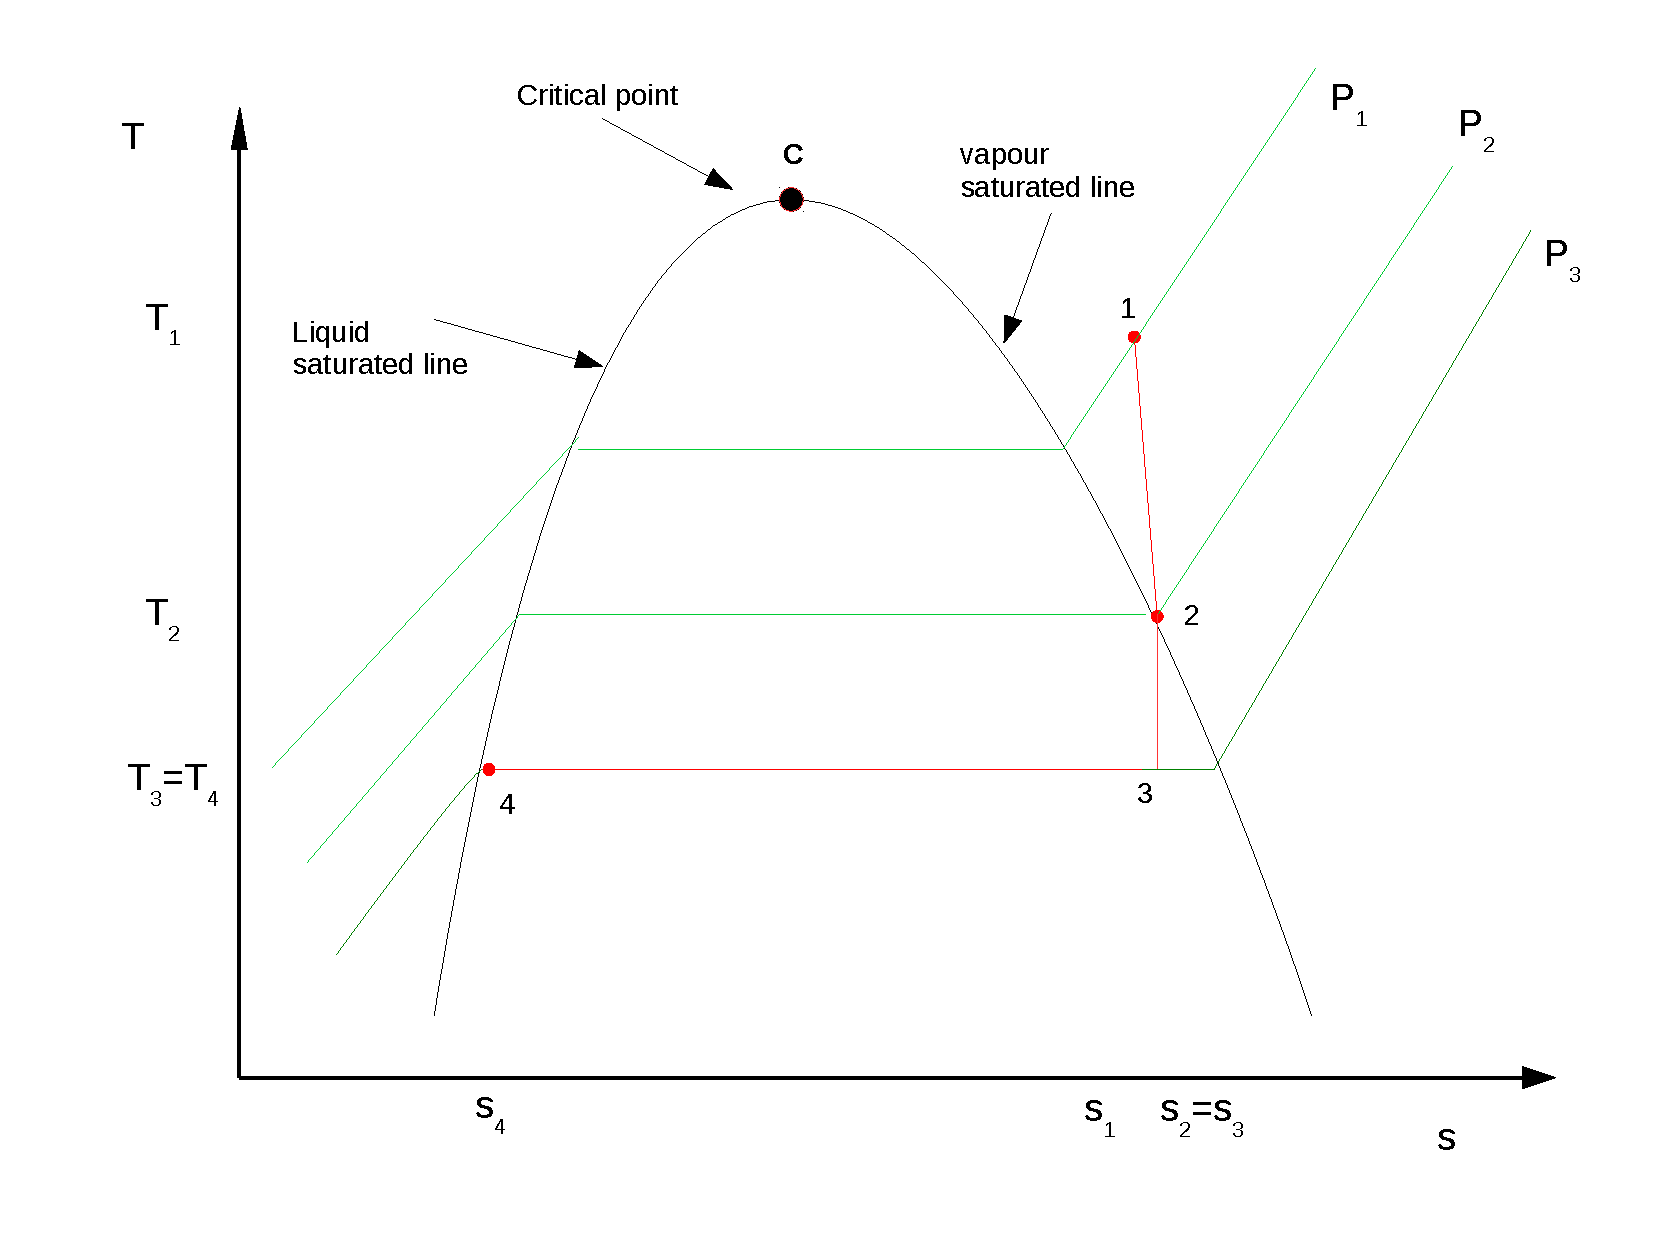
\includegraphics[width=.8\linewidth,clip]{./Pics/Exam_TSDiagram}
        \end{center}
        }
  \end{enumerate}
  In order to solve this problem, assume that brine has the same thermodynamic properties as water. Also, assume that ideal isentropic expansion and compression occurs at Turbine 2 and the Pump, respectively. Finally, assume that liquid brine behaves as an incompressible fluid.
\end{question} 
\clearpage


%%%
%%% Question 03 
%%%
\begin{question}
  \begin{enumerate}[a)]
%%%
%%% Nguyen (pg 128, Ex 5.3-1)
%%%
\item Calculate the bubble point pressure and vapour composition for a liquid mixture of 41.2 mol$\%$ of ethanol (1) and n-hexane (2) at 331 K. Given,
   \begin{eqnarray}
     && \ln{\gamma_{1}} = \frc{A}{\left(1+\frc{Ax_{1}}{Bx_{2}}\right)^{2}},\;\;\ln{\gamma_{2}} = \frc{A}{\left(1+\frc{Bx_{2}}{Ax_{1}}\right)^{2}} \text{ and } \nonumber \\
     && \nonumber\\
      && \ln{P_{i}^{sat}} = C_{i} + \frc{D_{i}}{T+E_{i}} \nonumber 
   \end{eqnarray}
   where
   \begin{displaymath}
     \begin{cases}
        A = 2.409, & B = 1.970 \\
        C_{1} = 16.1952, & C_{2} = 14.0568, \\
        D_{1} = -3423.53,& D_{2} = -2825.42,\\
        E_{1} = -55.7152, & E_{2} = -42.7089
     \end{cases}
   \end{displaymath}
   [P] = kPa and [T] = $\left[\text{D}_{i}\right]$ = $\left[\text{E}_{i}\right]$ = K.~\marks{10}

%========================
\solution{ At 331 K, the saturation pressures are $P_{1}^{sat}=$ 42.90 kPa and $P_{2}^{sat}=$ 7054 kPa.~\solmarks{2/10}

The liquid solution with $x_{1}=0.412$ and $x_{2}=0.588$ results in the following activity coefficient $\gamma_{1}=2.011$ and $\gamma_{2}=1.521$.~\solmarks{2/10}

The partial pressure of ethanol and n-hexane are,~\solmarks{2/10}
\begin{eqnarray}
P_{1} = x_{1}\gamma_{1}P_{1}^{sat} = 35.55\text{ kPa} \nonumber \\
P_{2} = x_{2}\gamma_{2}P_{2}^{sat} = 63.09\text{ kPa} \nonumber 
\end{eqnarray}
The bubble pressure is~\solmarks{2/10}
\begin{displaymath}
P =P_{1} + P_{2} = 98.64\text{ kPa}
\end{displaymath}
And the composition of the vapour phase is~\solmarks{2/10}
\begin{displaymath}
y_{1} = \frc{P_{1}}{P} = 0.360\;\;\text{ and } \;\; y_{2} = 0.640
\end{displaymath}

}
%========================

\item Given the van der Waals equation of state (vdW EOS),
     \begin{displaymath}
         P = \frc{RT}{V-b} - \frc{a}{V^{2}},
     \end{displaymath}
     Show that the vdW EOS can be expressed as a cubic polynomial equation in $Z$ (compressibility coefficient),
             \begin{displaymath}
                  Z^{3} -(1+B)Z^{2} +AZ -AB = 0,
             \end{displaymath}
             with $B=bP/(RT)$, $A=aP/(RT)^{2}$ and $R\left(=8.314\times 10^{-5}\frc{\text{bar.m}^{3}}{\text{mol.K}}\right)$ is the molar gas constant~\marks{10}
%==========================
\solution{We can rearrange the vdW EOS,~\solmarks{3/10}
\begin{displaymath}
   P = \frc{RT}{V-b} - \frc{a}{V^{2}} \Longrightarrow \frc{PV}{RT} = \frc{V}{V-b} - \frc{a}{RTV} = \frc{1}{1-\frc{b}{V}} - \frc{a}{RTV}
\end{displaymath}
Eliminating $V$ as $V=ZRT/P$,~\solmarks{2/10}
\begin{displaymath}
   Z = \left(1-\frc{bP}{ZRT}\right)^{-1} - \frc{aP}{Z\left(RT\right)^{2}} = \frc{ZRT}{ZRT-bP}-\frc{aP}{Z\left(RT\right)^{2}}
\end{displaymath}
Manipulating this expression,~\solmarks{3/10}
\begin{eqnarray}
   && Z^{2}R^{2}T^{2}\left(ZRT-bP\right) = Z^{2}\left(RT\right)^{3} - aP\left(ZRT-bP\right) \nonumber \\
   && Z^{3} - \frc{bP}{RT}Z^{2} - Z^{2} -\frc{aP}{\left(RT\right)^{2}}Z + ab\frc{P^{2}}{\left(RT\right)^{3}} = 0 \nonumber
\end{eqnarray}
with $B=bP/(RT)$, $A=aP/(RT)^{2}$,~\solmarks{2/7}
\begin{displaymath}
Z^{3} -(1+B)Z^{2} +AZ -AB = 0 
\end{displaymath}
} 
%
  \end{enumerate}
\end{question}

\clearpage


%%%
%%% Question 04
%%%
\begin{question}
  \begin{enumerate}[a)]
    \item Assuming that all species and their mixtures are ideal gases, derive an equation for the Gibbs energy as a function of the reaction coordinate for the reaction below at 1000K.
\begin{displaymath}
H_{2} + CO_{2} \Longleftrightarrow H_{2}O + CO
\end{displaymath}
Calculate the reaction coordinate, $\epsilon$, in the equilibrium.
Given $\Delta G_{f}^{\circ}$ $\left(\text{kJ.mol}^{-1}\right)$ at 1000K: (a) H$_{2}$O: -192.42, (b) CO: -200.24 and (c) CO$_{2}$: -395.79.~\marks{5}

%==========================
\solution{ The Gibbs energy can be expressed as
\begin{eqnarray}
G &=& \sum y_{i}G_{i} + RT\sum y_{i}\ln{y_{i}} \nonumber \\
G &=& \sum y_{i}\Delta G^{o}_{f,i} + RT\sum y_{i}\ln{y_{i}} \nonumber 
\end{eqnarray}
We can differentiate the total Gibbs energy as,
\begin{displaymath}
dG^{t} = d\left(n G\right) = n\frc{dG}{d\epsilon} + G\frc{d n}{d\epsilon} 
\end{displaymath} 
Assuming the system is closed and in equilibrium: $dn = 0$ and $\frc{dG}{d\epsilon}=0$. For 1 mole of H$_{2}$ and CO$_{2}$, the mole fraction of the gaseous species are~\solmarks{1/5}
\begin{displaymath}
y_{\text{H}_{2}}=\frc{1-\epsilon}{2} =y_{\text{CO}_{2}}\;\;\text{ and }\;\; y_{\text{H}_{2}\text{O}}=\frc{\epsilon}{2} =y_{\text{CO}}\
\end{displaymath}
Thus,~\solmarks{2/5}
\begin{eqnarray}
 G &=& \left(y_{H_{2}}\Delta G^{o}_{f,H_{2}} + y_{CO_{2}}\Delta G^{o}_{f,CO_{2}} + y_{H_{2}O}\Delta G^{o}_{f,H_{2}O} + y_{CO}\Delta G^{o}_{f,CO}\right) + \nonumber \\
    && RT\left(y_{H_{2}}\ln{y_{H_{2}}} + y_{CO_{2}}\ln{y_{CO_{2}}} + y_{H_{2}O}\ln{y_{H_{2}O}} + y_{CO}\ln{y_{CO}}\right) \nonumber \\
   &=&\left[\frc{1-\epsilon}{2}\Delta G^{o}_{f,CO_{2}} + \frc{\epsilon}{2}\left(\Delta G^{o}_{f,H_{2}O}+\Delta G^{o}_{f,CO}\right)\right] + RT\left[\left(1-\epsilon\right)\ln{\frc{1-\epsilon}{2}} + \epsilon\ln{\frc{\epsilon}{2}}\right]\nonumber
\end{eqnarray}
for $\Delta G^{o}_{f,H_{2}} = 0$. In the equilibrium $\frc{dG}{d\epsilon}=0$, therefore~\solmarks{2/5}
\begin{displaymath}
\frc{dG}{d\epsilon} = B-A + RT\left[\ln{\frc{\epsilon}{2}} - \ln{\frc{1-\epsilon}{2}}\right] = 0 \Longrightarrow \epsilon = 0.4531 
\end{displaymath}
with $A=\frc{-395790}{2}$ and $B=\frc{-192420-200240}{2}$.
}
%==========================
\item In the design of a new process, nitrogen dioxide $\left(\text{NO}_{2}\right)$ is produced through the decomposition of nitrogen tetroxide $\left(\text{N}_{2}\text{O}_{4}\right)$,
        \begin{displaymath}
           N_{2}O_{4} (g) \Longleftrightarrow 2 NO_{2} (g),
        \end{displaymath}
        The Gibbs energy of formation at 25$^{\circ}$C of both species are:
        \begin{displaymath}
           \left(\Delta G^{\circ}_{\text{f,298}}\right)_{N_{2}O_{4}} = 97.89 \text{ kJ.mol}^{-1} \text{ and } \left(\Delta G^{\circ}_{\text{f,298}}\right)_{NO_{2}} = 51.31 \text{ kJ.mol}^{-1}.
        \end{displaymath}
        The standard enthalpy of this reaction at 25$^{\circ}$C is 56.189 kJ.mol$^{-1}$. For such decomposition, three scenarios are considered to assess overall conversion:
        \begin{enumerate}[A.]
           \item Decomposition at 25$^{\circ}$C;
           \item Initial dilution with inert N$_{2}$ prior to the decomposition at 25$^{\circ}$C, where the initial concentration of $N_{2}O_{4}$ in the $N_{2}O_{4}-N_{2}$ mixture before the dissociation is 20 mol$\%$;
           \item Decomposition at 126.85$^{\circ}$C.
        \end{enumerate}
         Which scenario will lead to larger NO$_{2}$ production? Why?\marks{15}
%%%%%%%%%%%%%%%%%%%%%%%%%%%%%%%%%%%%%%%%%%%%%%%%%%%%%%%%%%%%%%%%%%       
         \solution{Larger production of NO$_{2}$ will depend on the conversion at equilibrium. Thus. let's calculate the equilibrium constant for each scenario:
           \begin{enumerate}[A.]
                 \item The equilibrium constant at 25$^{\circ}$C is
                    \begin{displaymath}
                        K = \exp\left(-\frc{\Delta G^{\circ}_{r,298}}{RT}\right) = \frc{a_{NO_{2}}^{2}}{a_{N_{2}O_{4}}} = \frc{\left(\frc{y_{NO_{2}}P}{P^{\circ}_{NO_{2}}}\right)^{2}}{\left(\frc{y_{N_{2}O_{4}}P}{P^{\circ}_{N_{2}O_{4}}}\right)} = \frac{\left(y_{NO_{2}}\right)^{2}}{\left(y_{N_{2}O_{4}}\right)},
                    \end{displaymath}
         where the standard Gibbs energy of reaction is~\solmarks{1/15}
         \begin{eqnarray}
           \Delta G^{\circ}_{r,298} &=& \sum\limits_{i}\nu_{i}\Delta G^{\circ}_{\text{f,298}} \nonumber \\
                             &=& (+2).\left(\Delta G^{\circ}_{\text{f,298}}\right)_{NO_{2}} + (-1).\left(\Delta G^{\circ}_{\text{f,298}}\right)_{N_{2}O_{4}} \nonumber \\ 
                             &=& 4730 \text{ J/mol}, \nonumber
         \end{eqnarray}
         and the equilibrium constant,~\solmarks{2/15}
         \begin{displaymath}
             K = \exp\left(-\frc{\Delta G^{\circ}_{r,298}}{RT}\right) = 0.1484 = \frac{\left(y_{NO_{2}}\right)^{2}}{\left(y_{N_{2}O_{4}}\right)}
         \end{displaymath}
         Composition and reaction coordinate are related through
         \begin{displaymath}
            y_{i} = \frc{n_{i,0} + \nu_{i}\varepsilon}{n_{0}+\nu\epsilon},
         \end{displaymath}
         where, assuming that the initial number of moles are $n_{N_{2}O_{4},0}=1$ and $n_{NO_{2},0}=0$, an $\nu= 2-1 = 1$,
         \begin{displaymath}
            y_{N_{2}O_{4}} = \frc{1-\varepsilon}{1+\varepsilon}\;\;\;\;\;\text{ and }\;\;\;\;\;\; y_{NO_{2}} = \frc{2\varepsilon}{1+\varepsilon},
         \end{displaymath}
         leading to
         \begin{displaymath}
             K = \frac{\left(y_{NO_{2}}\right)^{2}}{\left(y_{N_{2}O_{4}}\right)} = \frc{\left(\frc{2\varepsilon}{1+\varepsilon}\right)^{2}}{\left(\frc{1-\varepsilon}{1+\varepsilon}\right)} = 0.1484 \;\;\;\;\Longrightarrow\;\;\;\; \varepsilon = 0.1891
         \end{displaymath}
         Thus: $y_{NO_{2}} = 0.3181$ and $y_{N_{2}O_{4}} = 0.6819$.~\solmarks{2/15}

           \item Here, nitrogen is an inert species, \ie it is used to dilute the reactant gas, $N_{2}O_{4}$, but does not participate in the decomposition reaction, thus $\nu_{N_{2}}=0$.  The equilibrium constant was calculated previously as $K = 0.1484$ and 
         \begin{displaymath}
            y_{i} = \frc{n_{i,0} + \nu_{i}\varepsilon}{n_{0}+\nu\epsilon},
         \end{displaymath}
        The overall molar stoichiometric coefficient is $\nu= 2-1-0 = 1$, however the initial reactive composition is (assuming 1 mol of the reactant mixture) $n_{N_{2}O_{4},0} = 0.2$, $n_{N_{2},0} = 0.8$ and $n_{NO_{2},0}=0$.
         \begin{displaymath}
           y_{N_{2}O_{4}} = \frc{0.2-\varepsilon}{1+\varepsilon},\;\;\;\;\; y_{N_{2}} = \frc{0.8}{1+\varepsilon}\;\;\;\text{ and }\;\;\;y_{NO_{2}} = \frc{2\varepsilon}{1+\varepsilon}.
         \end{displaymath}
         Leading to~\solmarks{1/15} 
         \begin{displaymath}
             K = \frac{\left(y_{NO_{2}}\right)^{2}}{\left(y_{N_{2}O_{4}}\right)} = \frc{\left(\frc{2\varepsilon}{1+\varepsilon}\right)^{2}}{\left(\frc{0.2-\varepsilon}{1+\varepsilon}\right)} = 0.1484 \;\;\;\;\Longrightarrow\;\;\;\; \varepsilon = 0.0715,
         \end{displaymath}
         with equilibrium compositions of $y_{NO_{2}} = 0.1335$, $y_{N_{2}O_{4}} = 0.1199$ and $y_{N_{2}} = 0.7466$.~\solmarks{2/15} 

        \item In order to calculate composition at equilibrium, we need to calculate the equilibrium constant, $K$, at 126.85$^{\circ}$C (= 400 K) through the Van't Hoff equation,
\begin{displaymath}
    \frc{d\left(\ln{K}\right)}{dT} = \frc{\Delta H^{\circ}_{r}}{RT^{2}} \;\;\;\Longrightarrow \;\;\; \ln{\left(\frc{K(T)}{K(298.15\text{ K})}\right)} = \int\limits_{298.15\text{ K}}^{T}\frc{\Delta H^{\circ}_{r}}{RT^{2}}dT,
\end{displaymath}
with $K_{298.15\;K}=0.1484$. The standard heat of reaction is obtained from the fundamental enthalpy relation, $dH= C_{p}dT$, and~\solmarks{1/15}
\begin{displaymath}
     \Delta H^{\circ}_{r} = \summation[\nu_{i}\Delta H^{\circ}_{i,f}]{i}{} \;\;\;\Longrightarrow\;\;\; \int\limits_{\Delta H^{\circ}_{r,298.15}}^{\Delta H^{\circ}_{r,T}}d\left(\Delta H^{\circ}_{r}\right) = \int\limits_{298.15\text{ K}}^{T}\summation[\nu_{i} C_{p,i}]{i}{}dT.
\end{displaymath}
The first stage in this calculation is to obtain an expression for the right-hand side integration, \ie the summation term $\Delta C_{p}^{\circ} = \summation[\nu_{i} C_{p,i}]{i}{}$, using (for simplicity in the notation) $NO_{2}$:1 and $N_{2}O_{4}$:2,
\begin{eqnarray}
   \Delta C_{p}^{\circ} &=& \summation[\nu_{i} C_{p,i}]{i}{} = (+2) \left(a_{1}+b_{1}T+c_{1}T^{2}+d_{1}T^{3}\right) + (-1)\left(a_{2}+b_{2}T+c_{2}T^{2}+d_{2}T^{3}\right) \nonumber \\
                     &=& 12.804 - 7.239\times 10^{-2}T + 4.301\times 10^{-5} T^{2} + 15.732\times 10^{-9}T^{3} \nonumber 
\end{eqnarray}
And the integration becomes $\left(\text{with }\Delta H^{\circ}_{r,298.15} = 56189\text{ J.mol}^{-1}\right)$~\solmarks{1/15}
\begin{eqnarray}
    && \Delta H^{\circ}_{r}(T) - \Delta H^{\circ}_{r,298.15} = \int\Delta C_{p}^{\circ}dT \nonumber \\
    && \Delta H^{\circ}_{r}(T) = 56189 + 12.804 T - \frc{7.239\times 10^{-2}}{2}T^{2} + \frc{4.301\times 10^{-5}}{3}T^{3} + \frc{15.732\times 10^{-9}}{4}T^{4} \nonumber
\end{eqnarray}
Now, using the Van't Hoff equation,~\solmarks{1/15}
\begin{eqnarray}
  \ln{\left(\frc{K(T)}{K_{298.15\text{ K}}}\right)} &=& \int\limits_{298.15\text{ K}}^{T}\frc{\Delta H^{\circ}_{r}}{RT^{2}}dT \nonumber \\
                                                &=& \frc{1}{R}\int\limits_{298.15\text{ K}}^{T} \left[\frc{56189}{T^{2}} + \frc{12.804}{T} - \frc{7.239\times 10^{-2}}{2} + \frc{4.301\times 10^{-5}}{3}T + \right. \nonumber \\
                                                 && \hspace{3cm}\left.\frc{15.732\times 10^{-9}}{4}T^{2}\right]dT \nonumber \\
                                                &=& \frc{1}{R}\left[-\frc{56189}{T} + 12.804\ln{T} - \frc{7.239\times 10^{-2}}{2}T + \frc{4.301\times 10^{-5}}{6}T^{2} + \right. \nonumber \\
                                                &&\hspace{3cm}\left.\frc{15.732\times 10^{-9}}{12}T^{3}\right]_{298.15\text{ K}}^{T} \nonumber
\end{eqnarray}
Solving this integral for $T=400$ K leads to $K_{400\text{ K}} = 51.4338$~\solmarks{1/15}, with
         \begin{displaymath}
            y_{N_{2}O_{4}} = \frc{1-\varepsilon}{1+\varepsilon}\;\;\;\;\;\text{ and }\;\;\;\;\;\; y_{NO_{2}} = \frc{2\varepsilon}{1+\varepsilon},
         \end{displaymath}
         and
         \begin{displaymath}
             K = \frac{\left(y_{NO_{2}}\right)^{2}}{\left(y_{N_{2}O_{4}}\right)} = \frc{\left(\frc{2\varepsilon}{1+\varepsilon}\right)^{2}}{\left(\frc{1-\varepsilon}{1+\varepsilon}\right)}
         \end{displaymath}
         Leading to~\solmarks{2/15}
         \begin{displaymath}
             K_{400\text{ K}}   = 51.4331 \hspace{1.2cm} \Longrightarrow \varepsilon = 0.9632  \hspace{.35cm} \Longrightarrow \;\;  y_{NO_{2}} = 0.9813 \text{ and } y_{N_{2}O_{4}} = 0.0187
         \end{displaymath}
         
        Note that at low temperature, 250 K $\left(-23.15^{\circ}\text{C}\right)$, the production of nitrogen dioxide is fairly small (backward reaction), however as the temperature rises the forward reaction becomes dominant with 98.1$\%$ of NO$_{2}$ being produced at 400 K$\left(126.85^{\circ}\text{C}\right)$.

           \end{enumerate} 
         At room temperature conditions (A and B), the equilibrium constant is 0.1894 whereas at 400 K (C), it reaches 0.9632, \ie, most N$_{2}$O$_{4}$ is decomposed to produce NO$_{2}$. Thus, the best scenario is C.~\solmarks{1/15}
             }
          
         Given:
         \begin{displaymath}
           \Delta M_{r}^{\circ} = \summation[\nu_{i}\Delta M_{f,i}^{\circ}]{i=1}{\mathcal{C}}, \hspace{1cm} \text{ where }M=\left\{U,H,G,S,A\right\}, 
         \end{displaymath}
         and $\nu$ is the molar stoichiometric coefficient, and
         \begin{displaymath}
            \Delta H_{r}^{\circ}(T) - \Delta H_{r,25^{\circ}\text{C}}^{\circ} = \int \Delta C_{p}^{\circ}dT, \hspace{1cm} \text{ where } \Delta C_{p}^{\circ} = \summation[\nu_{i}C_{p,i}]{i=1}{\mathcal{C}}
         \end{displaymath}
     Heat capacity for both gases is expressed in polynomial form as,
  \begin{displaymath}
    C_{p} = a + bT + CT^{2} + dT^{3}, \;\;\;\;\left(\text{in J.mol}^{-1}\text{.K}^{-1}\right)
  \end{displaymath}
  where
  \begin{center}
    \begin{tabular}{ l | c c c c }
      \hline
                         &  $a$     &  $b\times 10^{-2}$  & $c\times 10^{-5}$  & $d\times 10^{-9}$ \\
                         &$\left(\text{J.mol}^{-1}\text{.K}^{-1}\right)$& $\left(\text{J.mol}^{-1}\text{.K}^{-2}\right)$& $\left(\text{J.mol}^{-1}\text{.K}^{-3}\right)$& $\left(\text{J.mol}^{-1}\text{.K}^{-4}\right)$ \\
      \hline
      NO$_{2}$             &  22.929 &      5.711          & -3.519            & 7.866 \\
      N$_{2}$O$_{4}$       &   33.054 &      18.661         &    -11.339        &  -- 
    \end{tabular}
  \end{center}
  \end{enumerate}
  
\end{question}

\clearpage


%%%
%%% Question 05 
%%%
\begin{question}
  \begin{enumerate}[a)]
    \item Figure~\ref{Figure:Fig1} shows a $P-xy$ phase diagram for an arbitrary binary mixture that is vaporised at constant temperature (M-z).
      \begin{figure}[h]
        \begin{center}
          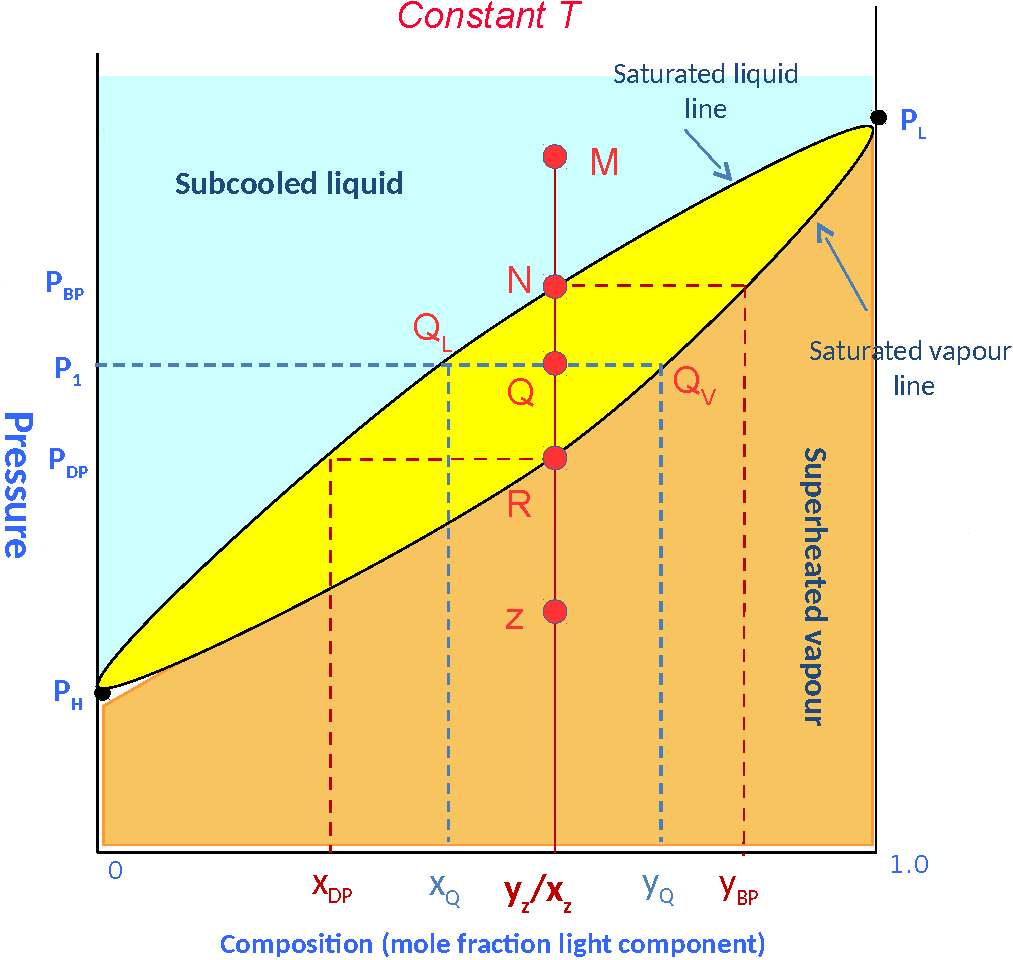
\includegraphics[width=.5\linewidth,clip]{./Pics/VLE_Pxy_Diagram3b}
          \caption{VLE for binary mixture: P-xy diagram at constant temperature.}\label{Figure:Fig1}
        \end{center}
      \end{figure}
      Determine (i)-(ix) from Table~\ref{Table:Tab1}.\marks{10}
      \begin{table}[h]
        \begin{center}
          \begin{tabular}{||c| c | c | c | c ||}
            \hline\hline
            {\bf Coordinate} & {\bf Pressure} & {\bf Fluid State} & $\mathbf{x}_{1}$ & $\mathbf{y}_{1}$ \\
            \hline
                 M           &   --           &   subcooled liquid & $x_{1}=x_{z}$    & $y_{1}=0$        \\
                 N           &bubble point $\left(P_{BP}\right)$&--& (i)             & (ii)            \\
                 Q           &  --            &     (iii)          & (iv)             & (v)            \\
                 R           &  (vi)          &     --             & (vii)             & (viii)            \\
                 z           &  --           &     (ix)            & (x)         &  --            \\                 
            \hline\hline
          \end{tabular}
        \end{center}
        \caption{Properties of $P-xy$ phase diagram}\label{Table:Tab1}
      \end{table}
      \solution{
        \begin{enumerate}[(i)]
           \item $x_{1}=x_{z}$;\solmarks{1/10}
           \item $y_{1}=y_{BP}$;\solmarks{1/10}
           \item vapour-liquid mixture;\solmarks{1/10}
           \item $x_{1}=x_{Q}$;\solmarks{1/10}
           \item $y_{1}=y_{Q}$;\solmarks{1/10}
           \item dew point $\left(P_{DP}\right)$;\solmarks{1/10}
           \item $x_{1}=x_{DP}$;\solmarks{1/10}
           \item $y_{1}=y_{z}$;\solmarks{1/10}
           \item superheated vapour;\solmarks{1/10}
           \item $x_{1}=0$;\solmarks{1/10}
        \end{enumerate}
        }
        
%====================================================
%%% Moran & Shapiro (Example 11.5)      
     \item Using the Redlich-Kwong equation of state, develop algebraic expressions for changes in specific entropy $\left(s_{2}-s_{1}\right)$ and internal energy $\left(u_{2}-u_{1}\right)$ of a gas between two states at the same temperature, \ie $T_{1}=T_{2}$, and pressures $P_{1}$ and $P_{2}$.\marks{10}
%====================
        \solution{The RK EOS is explicit in pressure,
           \begin{displaymath}
             P = \frc{R T}{v-b} - \frc{a}{v\sqrt{T}\left(v+b\right)},
           \end{displaymath}
           and in order to obtain $u_{2}-u_{1}$, $s_{2}-s_{1}$ we should integrate
           \begin{displaymath}
             \begin{cases}
               ds = \frc{C_{v}}{T}dT + \Partial[P]{T}{v}dv & \\
               du = C_{v}dT + \left[T\Partial[P]{T}{v}-P\right]dv & \\
             \end{cases}
           \end{displaymath}
          At the isotherm $T_{1}=T_{2}$,\solmarks{2/10}
           \begin{displaymath}
             \begin{cases}
               s_{2}-s_{1} = \displaystyle\int\limits_{v_{1}}^{v_{2}} \Partial[P]{T}{v}dv, & \\
               u_{2}-u_{1} = \displaystyle\int\limits_{v_{1}}^{v_{2}} \left[T\Partial[P]{T}{v}-P\right]dv. & \\
             \end{cases}
           \end{displaymath}
           The limits for the integrals are the specific volumes $v_{1}$ and $v_{2}$ at the two states under consideration. Using $P_{1}$ and $P_{2}$ and the known temperature, $T_{1}=T_{2}=T$, these specific volumes should be readily obtained from the RK EOS. Before integrating, we need to solve the partial differential $\Partial[P]{T}{v}$ for the RK EOS,
           \begin{displaymath}
             \Partial[P]{T}{v} = \frc{R}{v-b} + \frc{a}{2v\left(v+b\right)T^{3/2}}.
           \end{displaymath}
           Now solving for the change in entropy,\solmarks{3/10}
           \begin{eqnarray}
             s_{2}-s_{1} &=& \displaystyle\int\limits_{v_{1}}^{v_{2}} \left[\frc{R}{v-b} + \frc{a}{2v\left(v+b\right)T^{3/2}}\right]dv \nonumber \\
                        &=& R \ln{\left(\frc{v_{2}-b}{v_{1}-b}\right)} + \frc{a}{2bT^{3/2}}\left[\ln{\frc{v_{2}}{v_{1}}}-\ln{\frc{v_{2}+b}{v_{1}+b}}\right] \nonumber \\
                        &=& R \ln{\left(\frc{v_{2}-b}{v_{1}-b}\right)} + \frc{a}{2bT^{3/2}}\ln{\frc{v_{2}\left(v_{1}+b\right)}{v_{1}\left(v_{2}+b\right)}}.\nonumber
           \end{eqnarray}
           For the change in internal energy, the term in bracket\solmarks{2/10}
           \begin{displaymath}
             \left[T\Partial[P]{T}{v}-P\right] = \frc{3a}{2v\left(v+b\right)T^{1/2}},
           \end{displaymath}
           need to be integrated from $v_{1}$ to $v_{2}$,\solmarks{3/10}
           \begin{eqnarray}
             u_{2}-u_{1} &=& \displaystyle\int\limits_{v_{1}}^{v_{2}} \frc{3a}{2v\left(v+b\right)T^{1/2}}dv \nonumber \\
                        &=& \frc{3a}{2bT^{1/2}}\left[\ln{\frc{v_{2}}{v_{1}}} - \ln{\frc{v_{2}+b}{v_{1}+b}}\right] \nonumber \\
                        &=& \frc{3a}{2bT^{1/2}}\left[\ln{\frc{v_{2}\left(v_{1}+b\right)}{v_{1}\left(v_{2}+b\right)}}\right].\nonumber
           \end{eqnarray}
        }
%====================================================
  \end{enumerate}
  
\end{question}


\vfill
\paperend



\vfill 



\begin{comment}
{
  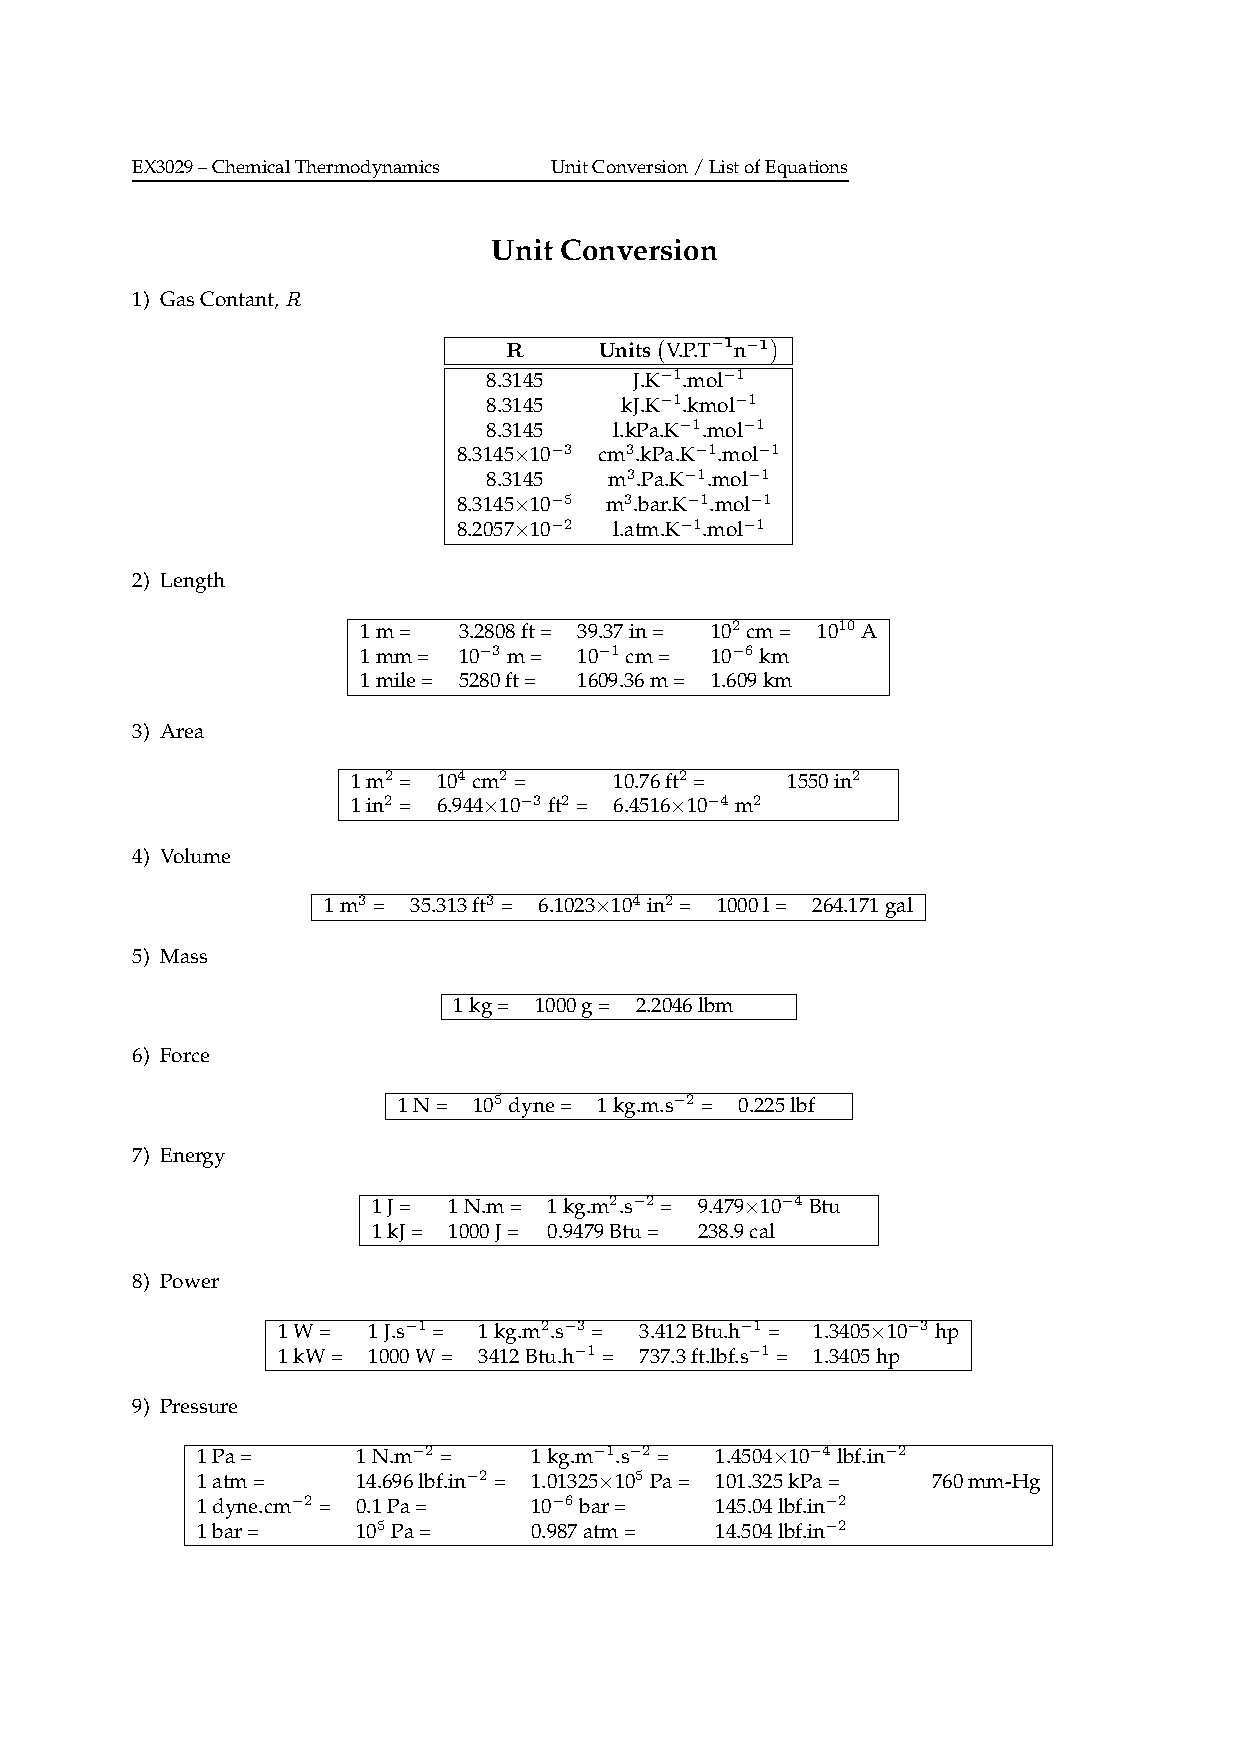
\includepdf[pages=-,fitpaper]{./Pics/EquationsList}
  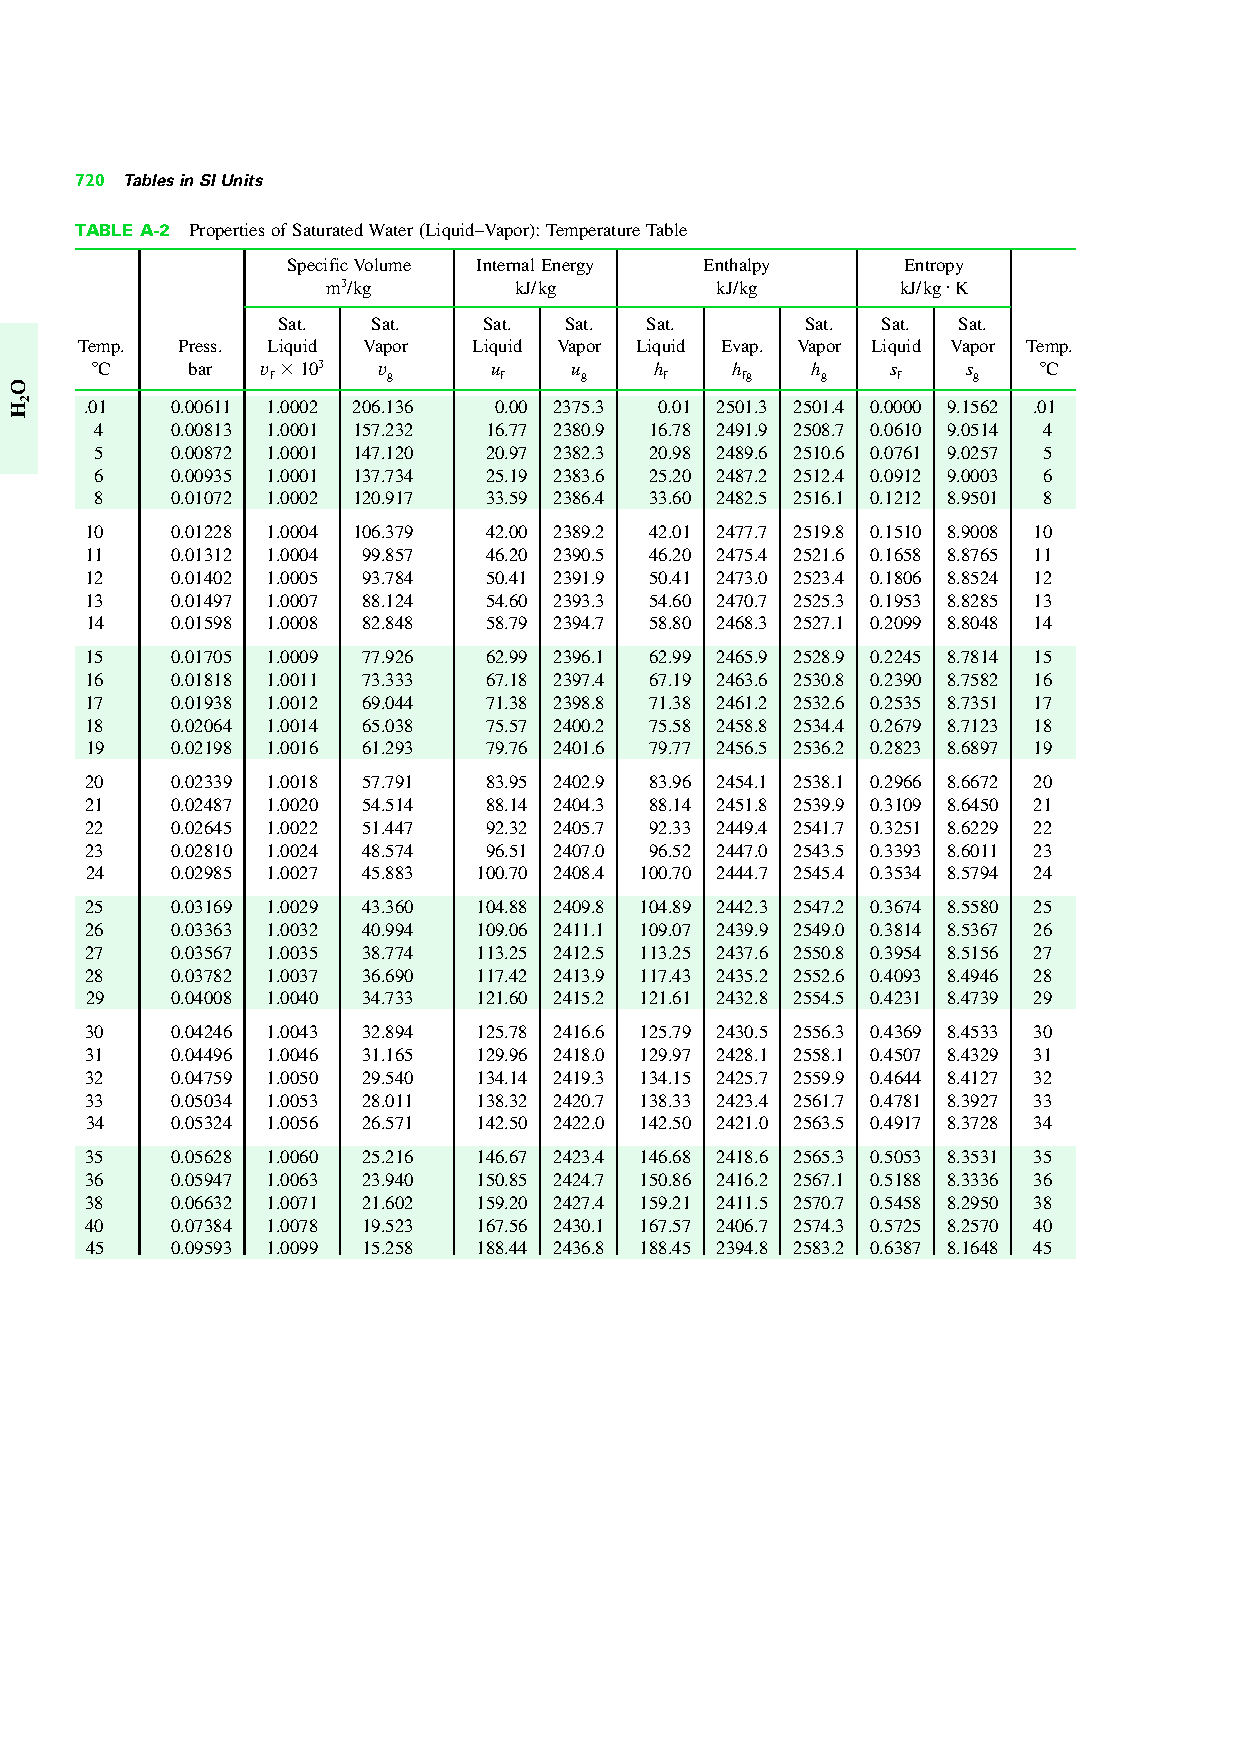
\includepdf[pages=-,fitpaper]{./Appendix4Exams/Tables/SatProp_H2O}
}
\end{comment}



\end{document}
